
\documentclass[12pt,a4paper]{article}

% Encodage et langue
\usepackage[utf8]{inputenc}
\usepackage[T1]{fontenc}
\usepackage[french]{babel}

% Packages mathématiques et mise en page
\usepackage{amsmath,amssymb}
\usepackage{graphicx}
\usepackage{float}
\usepackage{geometry}
\usepackage{xcolor}
\usepackage{listings}
\usepackage{hyperref}

% Marges
\geometry{margin=2.5cm}

% Configuration des blocs de code Python
\lstset{
    language=Python,
    basicstyle=\ttfamily\small,
    keywordstyle=\color{blue},
    commentstyle=\color{gray},
    stringstyle=\color{red},
    breaklines=true,
    frame=single,
    numbers=left,
    numberstyle=\tiny,
    showstringspaces=false
}

% Informations du rapport

% Informations du rapport
\title{
    \textbf{Compte rendu de TP}\\[0.3cm]
    \Large Importance Sampling
}

\author{
    Narjah Fatimetou\\
    Benloughmari Mohamed\\[0.3cm]
    ENSTA Paris
}

\date{15 octobre 2026}

\begin{document}

\maketitle

\section{Introduction}

L'objectif de ce TP est d'étudier différentes méthodes
de Monte-Carlo pour approximer une intégrale et de comparer
leur précision ainsi que leur coût de calcul.

On considère l'intégrale :
\[
\mu = \int_0^1 \cos\left(\frac{\pi x}{2}\right)\,dx.
\]

Sa valeur exacte est :
\[
\mu = \frac{2}{\pi} \approx 0{,}63662.
\]

Dans un premier temps, nous étudions la méthode de
Monte-Carlo classique. Nous considérons ensuite la méthode
d'échantillonnage d'importance (\textit{Importance Sampling}),
qui consiste à utiliser une densité de probabilité adaptée
afin de réduire la variance de l'estimateur.

Enfin, nous comparons les résultats théoriques aux résultats
obtenus par simulation numérique, étudions la convergence
des estimateurs et vérifions numériquement le théorème
central limite.

% La première partie du TP commence ici :
\section{Méthode de Monte-Carlo classique}

\subsection{Variance théorique}

Pour $X\sim\mathcal{U}([0,1])$ et
$g(x)=\cos\left(\frac{\pi x}{2}\right)$, on a :
\[
\mathbb{E}[g(X)]=\frac{2}{\pi},
\qquad
\mathbb{E}[g(X)^2]=\frac{1}{2}.
\]

Ainsi,
\[
\operatorname{Var}(g(X))
=\frac{1}{2}-\frac{4}{\pi^2}
\approx 0{,}094715.
\]

La variance de l'estimateur de Monte-Carlo est donc :
\[
\operatorname{Var}(\widehat{\mu}_N)
=\frac{1}{N}\left(\frac{1}{2}-\frac{4}{\pi^2}\right).
\]

Pour $N=50$, on obtient :
\[
\boxed{\operatorname{Var}(\widehat{\mu}_{50})
\approx 0{,}0018943.}
\]

\subsection{Estimation empirique de la variance}

Pour $N=50$, nous réalisons $M=100$ simulations indépendantes.
La moyenne et la variance empiriques des estimations sont :

\[
\overline{\mu}=0{,}638955,
\qquad
V_{\mathrm{emp}}=0{,}00141784.
\]

La variance théorique étant
\[
V_{\mathrm{th}}=0{,}00189431,
\]
on constate que la variance empirique est du même ordre de grandeur,
mais présente un écart dû aux fluctuations aléatoires et au nombre
limité de simulations.

\subsection{Étude de la convergence en fonction de $N$}

D'après la loi des grands nombres, l'estimateur
$\widehat{\mu}_N$ converge vers $\mu=2/\pi$ lorsque
$N$ augmente.

Le graphique compare l'erreur quadratique moyenne (RMSE)
empirique à l'erreur théorique :
\[
\operatorname{RMSE}(\widehat{\mu}_N)
=\sqrt{\frac{\operatorname{Var}(g(X))}{N}}.
\]

\begin{figure}[H]
    \centering
    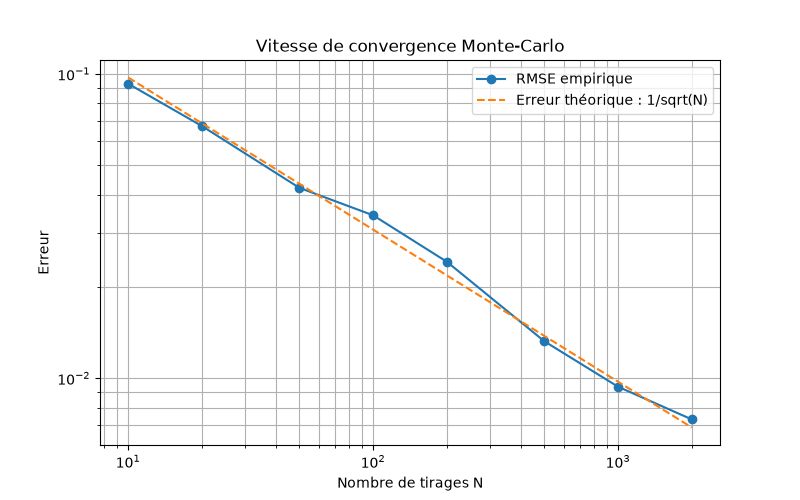
\includegraphics[width=0.85\textwidth]{convergence.png}
    \caption{Convergence de l'estimateur de Monte-Carlo en fonction du nombre de tirages $N$.}
    \label{fig:convergence}
\end{figure}

On observe que l'erreur diminue lorsque le nombre de tirages
augmente et que la courbe empirique suit globalement la
courbe théorique. L'erreur évolue en $1/\sqrt{N}$ :
pour diviser l'erreur par deux, il faut multiplier $N$ par quatre.

\subsection{Vérification numérique du TCL}

Pour $N=50$, nous réalisons $M=10\,000$ simulations
indépendantes. Chaque estimation est centrée et réduite :
\[
Z_N=\frac{\widehat{\mu}_N-\mu}
{\sqrt{\operatorname{Var}(g(X))/N}}.
\]

D'après le théorème central limite, $Z_N$ suit approximativement
une loi normale standard $\mathcal{N}(0,1)$.

La simulation donne :
\[
\mathbb{E}_{\mathrm{emp}}[Z_N]\approx -0{,}045,
\qquad
\operatorname{Var}_{\mathrm{emp}}(Z_N)\approx 0{,}850.
\]

L'histogramme obtenu présente une forme globalement en cloche,
compatible avec une approximation normale. La moyenne empirique
est proche de $0$ et la variance proche de $1$ ; les écarts
observés sont dus aux fluctuations de la simulation.

\begin{figure}[H]
    \centering
    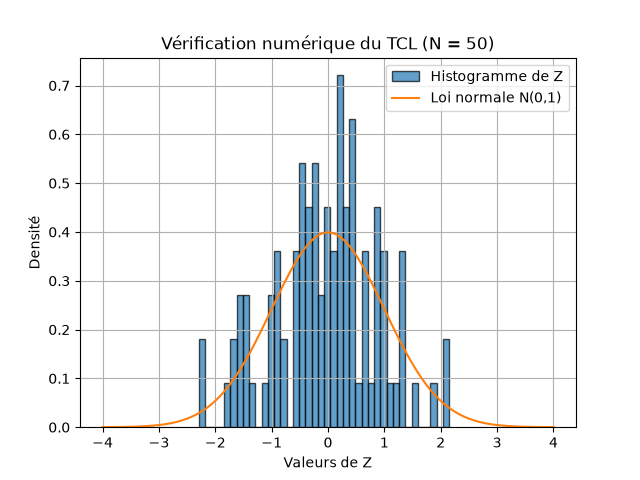
\includegraphics[width=0.8\textwidth]{tcl_monte_carlo.png}
    \caption{Vérification numérique du TCL pour Monte-Carlo classique avec $N=50$.}
    \label{fig:tcl-mc}
\end{figure}

\section{Importance sampling}

\subsection{1. Détermination de la densité d'importance optimale}

La densité d'importance optimale est proportionnelle à
$g(x)q(x)$ et s'écrit :
\[
\boxed{
\widetilde q_{\mathrm{opt}}(x)
=\frac{g(x)q(x)}{\mu}
=\frac{\pi}{2}\cos\left(\frac{\pi x}{2}\right).
}
\]

Cette densité minimise la variance de l'estimateur. Elle
n'est généralement pas directement utilisable, car sa
normalisation dépend de $\mu$, l'intégrale que l'on cherche
à estimer.

\subsection{2. Développement limité au voisinage de $0$}

Le développement limité de $\cos(u)$ au voisinage de $0$ est :
\[
\cos(u)=1-\frac{u^2}{2}+o(u^2).
\]

En prenant $u=\frac{\pi x}{2}$, on obtient :
\[
\boxed{
g(x)=\cos\left(\frac{\pi x}{2}\right)
=1-\frac{\pi^2x^2}{8}+o(x^2).
}
\]

Ainsi, une approximation au voisinage de $0$ est
$g(x)\approx 1-\frac{\pi^2x^2}{8}$.

\subsection{3. Validité de l'approximation comme densité}

On ne peut pas utiliser directement
$1-\frac{\pi^2x^2}{8}$ comme densité sur $[0,1]$,
car une densité doit être positive ou nulle partout.
Or, en $x=1$ :
\[
1-\frac{\pi^2}{8}<0.
\]

Cette approximation ne satisfait donc pas la condition
de positivité d'une densité.

\subsection{4. Normalisation de la densité proposée}

On considère une densité de la forme
$\widetilde q(x)=C(1-x^2)$ sur $[0,1]$.
Pour qu'elle soit une densité de probabilité, il faut :
\[
\int_0^1 C(1-x^2)\,dx=1.
\]

Ainsi,
\[
C\left[x-\frac{x^3}{3}\right]_0^1=1
\quad\Longrightarrow\quad
C\frac{2}{3}=1.
\]

Par conséquent,
\[
\boxed{C=\frac{3}{2}},
\qquad
\boxed{\widetilde q(x)=\frac{3}{2}(1-x^2)}.
\]

\subsection{Tracé et comparaison des densités}

Nous traçons les trois fonctions $q(x)$, $g(x)q(x)$ et
$\widetilde q(x)$ sur $[0,1]$, avec :
\[
q(x)=1,\qquad
g(x)q(x)=\cos\left(\frac{\pi x}{2}\right),
\qquad
\widetilde q(x)=\frac{3}{2}(1-x^2).
\]

La densité uniforme $q(x)$ est constante, tandis que
$g(x)q(x)$ et $\widetilde q(x)$ sont décroissantes et
s'annulent en $x=1$. La densité d'importance proposée
est plus élevée que $g(x)q(x)$ sur une grande partie
de l'intervalle. Elle permet ainsi de générer davantage
d'échantillons près de $x=0$, où $g(x)q(x)$ est élevée.

\begin{figure}[H]
    \centering
    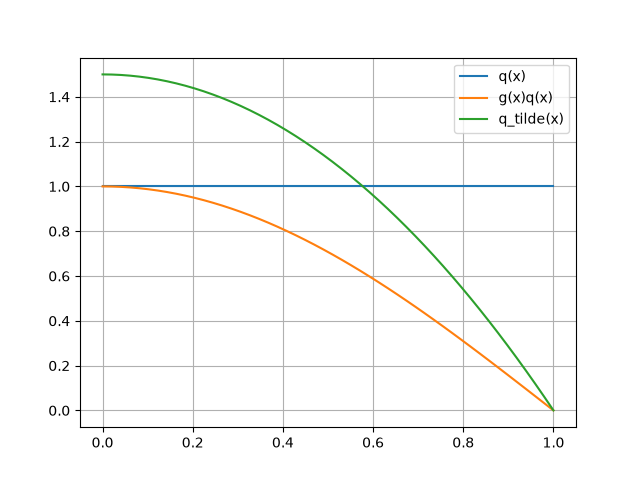
\includegraphics[width=0.8\textwidth]{densites.png}
    \caption{Comparaison de $q(x)$, $g(x)q(x)$ et $\widetilde q(x)$.}
    \label{fig:densites}
\end{figure}


\section{Importance sampling avec acceptation-rejet}

\subsection{Détermination de la densité d'importance}

Le développement limité de $g(x)=\cos(\pi x/2)$ au voisinage
de $0$ donne :
\[
g(x)\approx 1-\frac{\pi^2x^2}{8}.
\]

Cette approximation peut devenir négative sur $[0,1]$.
On propose donc une densité de la forme
$\widetilde q(x)=C(1-x^2)$, où $C$ est une constante.

La condition de normalisation impose :
\[
\int_0^1 C(1-x^2)\,dx=1
\quad\Longrightarrow\quad C=\frac32.
\]

La densité d'importance utilisée est donc :
\[
\boxed{\widetilde q(x)=\frac32(1-x^2).}
\]

\subsection{Calcul de la variance théorique}

L'estimateur d'importance sampling repose sur les poids
\[
H(x)=\frac{g(x)q(x)}{\widetilde q(x)}
=\frac{\cos(\pi x/2)}{\frac32(1-x^2)}.
\]

Sa variance théorique est :
\[
\operatorname{Var}(\widehat{\mu}_N)
=\frac{1}{N}
\left[
\int_0^1\frac{g(x)^2q(x)^2}{\widetilde q(x)}\,dx
-\mu^2
\right].
\]

L'intégrale est calculée numériquement avec Python.
Pour $N=50$, on obtient :
\[
\boxed{
\operatorname{Var}(\widehat{\mu}_{50})
\approx 1{,}98166\times10^{-5}.
}
\]


\subsection{Méthode d'acceptation-rejet}

Pour générer des échantillons suivant la densité
$\widetilde q(x)=\frac32(1-x^2)$, on propose
$X\sim\mathcal U([0,1])$ et $U\sim\mathcal U([0,1])$,
puis on accepte $X$ si :
\[
U<1-X^2.
\]

La probabilité d'acceptation théorique est :
\[
P_a=\frac{1}{3/2}\int_0^1
\frac32(1-x^2)\,dx
=\boxed{\frac23\approx 0{,}6667}.
\]

Pour $M=10^5$ propositions, la simulation donne :
\[
P_{a,\mathrm{emp}}=0{,}66903,
\qquad
\text{écart}=0{,}00236.
\]

Au total, $66\,903$ valeurs ont été acceptées.
La probabilité empirique est proche de la valeur théorique,
ce qui valide numériquement la méthode d'acceptation-rejet.

\subsection{Estimation empirique de la variance}

Nous réalisons $M=10\,000$ simulations indépendantes,
avec $N=50$ échantillons acceptés pour chaque estimation.
La variance empirique est calculée à partir des estimations
$\widehat{\mu}_N^{(m)}$ :
\[
\widehat V_{\mathrm{emp}}
=\frac{1}{M-1}\sum_{m=1}^{M}
\left(\widehat{\mu}_N^{(m)}-\overline{\mu}\right)^2.
\]

Les résultats obtenus sont :
\[
\overline{\mu}=0{,}636624,
\qquad
\widehat V_{\mathrm{emp}}\approx 2{,}00982\times10^{-5}.
\]

La variance empirique est proche de la variance théorique
$1{,}98166\times10^{-5}$. Cela confirme la cohérence
des résultats numériques.

\section{Comparaison des deux méthodes}

\subsection{Comparaison théorique et empirique des variances}

Pour $N=50$, les variances théoriques des deux méthodes sont :
\[
V_{\mathrm{MC}} \approx 1{,}8943\times10^{-3},
\qquad
V_{\mathrm{IS}} \approx 1{,}9817\times10^{-5}.
\]

Le rapport des variances vaut :
\[
\boxed{
\frac{V_{\mathrm{MC}}}{V_{\mathrm{IS}}}
\approx 95{,}6.
}
\]

L'échantillonnage d'importance présente donc une variance
environ 96 fois plus faible que Monte-Carlo classique.
Pour une même précision, il nécessite théoriquement
environ 96 fois moins d'échantillons.

Les simulations confirment ce résultat :
\[
V_{\mathrm{MC,emp}}\approx 1{,}4178\times10^{-3},
\qquad
V_{\mathrm{IS,emp}}\approx 2{,}0098\times10^{-5}.
\]

\subsection{Validation numérique du théorème central limite}

Pour les deux méthodes, on centre et réduit les estimations :
\[
Z=\frac{\widehat{\mu}_N-\mu}
{\sqrt{\operatorname{Var}(\widehat{\mu}_N)}}.
\]

D'après le théorème central limite, la variable $Z$ suit
approximativement une loi normale standard $\mathcal{N}(0,1)$
pour $N=50$.

Les histogrammes obtenus par simulation sont globalement
proches de la densité de la loi normale standard. Cette
observation est cohérente avec le théorème central limite
pour les deux méthodes.

\begin{figure}[H]
    \centering
    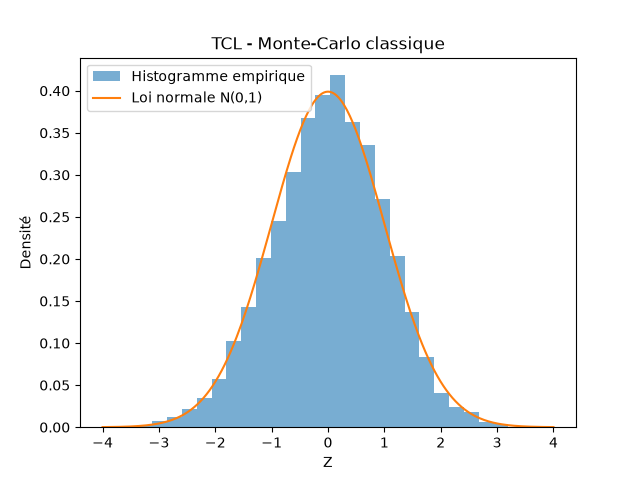
\includegraphics[width=0.8\textwidth]{TCL_montecarlo.png}
    \caption{Validation du TCL pour Monte-Carlo classique.}
    \label{fig:tcl-mc}
\end{figure}

\begin{figure}[H]
    \centering
    \includegraphics[width=0.8\textwidth]{tcl_is.png}
    \caption{Validation du TCL pour l'échantillonnage d'importance.}
    \label{fig:tcl-is}
\end{figure}

Pour obtenir une même précision, le nombre de tirages
nécessaires est proportionnel à la variance de l'estimateur.
Le rapport des budgets théoriques est donc :

\[
\frac{N_{\mathrm{MC}}}{N_{\mathrm{IS}}}
=\frac{V_{\mathrm{MC}}}{V_{\mathrm{IS}}}
\approx 95{,}6.
\]

Ainsi, l'échantillonnage d'importance nécessite théoriquement
environ 96 fois moins d'échantillons pour obtenir une
précision équivalente, sans tenir compte du coût de génération
des échantillons.

\subsection{Variance avec la densité d'importance optimale}

La densité d'importance optimale est :
\[
\widetilde q_{\mathrm{opt}}(x)
=\frac{g(x)q(x)}{\mu}
=\frac{\pi}{2}\cos\left(\frac{\pi x}{2}\right).
\]

Avec cette densité, le poids de l'estimateur est constant :
\[
\frac{g(x)q(x)}{\widetilde q_{\mathrm{opt}}(x)}
=\mu.
\]

L'estimateur vaut donc exactement $\mu$ pour chaque
simulation. Les résultats numériques donnent :
\[
\overline{\mu}=0{,}636620,
\qquad V_{\mathrm{emp}}=0.
\]

La variance est nulle, car la densité optimale nécessite
de connaître $\mu$, précisément la quantité à estimer.
Elle est donc généralement inutilisable directement.


\subsection{Importance sampling avec $\widetilde q(x)=2(1-x)$}

On considère la densité :
\[
\widetilde q(x)=2(1-x),\qquad x\in[0,1].
\]

Sa fonction de répartition est
\[
F(x)=\int_0^x 2(1-t)\,dt=2x-x^2.
\]

En posant $U=F(X)$ avec $U\sim\mathcal U([0,1])$,
l'inversion de la fonction de répartition donne :
\[
\boxed{X=1-\sqrt{1-U}.}
\]

La variance théorique de l'estimateur pour $N=50$ est :
\[
V_{\mathrm{IS}}\approx 1{,}35694\times10^{-4}.
\]

La simulation donne :
\[
\overline{\mu}_{\mathrm{emp}}=0{,}636706,
\qquad
V_{\mathrm{emp}}\approx 1{,}41963\times10^{-4}.
\]

Pour comparaison, la variance de Monte-Carlo classique
est $V_{\mathrm{MC}}\approx 1{,}89431\times10^{-3}$.
La variance de cette méthode d'importance est donc plus
faible que celle de Monte-Carlo classique.

\end{document}
